% !TeX program = pdfLaTeX
\documentclass[smallextended]{svjour3}       % onecolumn (second format)
%\documentclass[twocolumn]{svjour3}          % twocolumn
%
\smartqed  % flush right qed marks, e.g. at end of proof
%
\usepackage{amsmath}
\usepackage{graphicx}
\usepackage[utf8]{inputenc}

\usepackage[hyphens]{url} % not crucial - just used below for the URL
\usepackage{hyperref}
\providecommand{\tightlist}{%
  \setlength{\itemsep}{0pt}\setlength{\parskip}{0pt}}

%
% \usepackage{mathptmx}      % use Times fonts if available on your TeX system
%
% insert here the call for the packages your document requires
%\usepackage{latexsym}
% etc.
%
% please place your own definitions here and don't use \def but
% \newcommand{}{}
%
% Insert the name of "your journal" with
% \journalname{myjournal}
%

%% load any required packages here



\journalname{Biological Invasions}
\usepackage{natbib}
\usepackage{float}
\floatplacement{figure}{H}

\begin{document}

\title{Spatial variation in allometric growth of invasive lionfish has
management implications }


    \titlerunning{Lionfish allometric growth}

\author{  Juan Carlos Villaseñor-Derbez \and  Sean Fitzgerald \and  }

    \authorrunning{ Villaseñor-Derbez \& Fitzgerald }

\institute{
        Juan Carlos Villaseñor-Derbez \at
     Bren School of Environmental Science and Management, University of
 California Santa Barbara, Santa Barbara, California, United States,
 93117 \textbar{} ORCID: 0000-0003-1245-589X \\
     \email{\href{mailto:jvillasenor@bren.ucsb.edu}{\nolinkurl{jvillasenor@bren.ucsb.edu}}}  %  \\
%             \emph{Present address:} of F. Author  %  if needed
    \and
        Sean Fitzgerald \at
     Bren School of Environmental Science and Management, University of
 California Santa Barbara, Santa Barbara, California, United States,
 93117 \\
     %  \\
%             \emph{Present address:} of F. Author  %  if needed
    \and
    }

\date{Received: date / Accepted: date}
% The correct dates will be entered by the editor


\maketitle

\begin{abstract}
Lionfish (\textit{Pterois volitans / miles}) are an invasive species in
the Western Atlantic and the Caribbean. Improving management of invasive
lionfish populations requires accurate total biomass estimates, which
depend on accurate estimates of allometric growth. Sedentary species
like lionfish often exhibit high levels of spatial variation in life
history characterstics. We review 17 published length-weight
relationships for lionfish taken throughout their invasive range and
found substantial regional differences in allometric growth parameters.
The spatial pattern we observed is consistent with findings from other
studies focusing on genetics or age-at-length. We show that the use of
\textit{ex situ} parameters can result in up to a threefold under- or
overestimation of total weight, but using parameters from nearby regions
reduces this error. These findings can have major implications for
management in terms of predicting effects on local ecosystems,
evaluating the effectiveness of removal programs, or estimating biomass
available for harvest.
\\
\keywords{
        Lionfish \and
        invasive species \and
        length-weight \and
        allometric growht \and
        regional variations \and
    }


\end{abstract}


\def\spacingset#1{\renewcommand{\baselinestretch}%
{#1}\small\normalsize} \spacingset{1}


\section{Introduction}\label{introduction}

Lionfish (\emph{Pterois volitans/miles} complex) are an invasive species
in the western Atlantic and Caribbean Sea, likely introduced through
liberation of aquarium-kept organisms \citep{betancurr_2011}. They are
the first invasive marine vertebrates established along the North
Atlantic Caribbean coasts
\citep{schofield_2009,schofield_2010,sabidoitza_2016} and their presence
has been labeled as a major marine invasion because they threaten local
biodiversity, spread rapidly, and are difficult to manage
\citep{hixon_2016}. Lionfish have established invasive populations in
coral reefs, estuaries, mangroves, hard-bottomed areas, and mesophotic
reefs
\citep{barbour_2010,jud_2011,muoz_2011,claydon_2012,andradibrown_2017,gress_2017}.

A substantial amount of research describes lionfish impacts throughout
its invaded range. A meta-analysis by \citet{peake_2018} showed that
invasive lionfish prey on at least 167 different species across the
tropical and temperate North Atlantic. Their feeding behavior and high
consumption rates can reduce recruitment and population sizes of native
reef-fish species, and can further endanger reef fish
(\citet{green_2012,rocha_2015}; but see \citet{hackerott_2017}). For
example, field experiments by \citet{albins_2008} showed that lionfish
establishment led to reduced recruitment of native fishes by nearly 80\%
over a five week period in Florida. \citet{green_2012} reported that
prey fish biomass declined by 65\% over two years as lionfish biomass
increased along Bahamian coral reefs. Their trophic impacts can be
minimized if local lionfish biomass is controlled by culling
\citep{ariasgonzalez_2011}.

Governments and non-profit organizations have sought to reduce lionfish
densities through removal programs and incentivizing its consumption
\citep{chin_2016}. In some cases, these have shown to significantly
reduce --but not quite eliminate-- lionfish abundances at local scales
\citep{deleon_2013,sandel_2015}. Complete eradication of lionfish
through fishing is unlikely because of their rapid recovery rates and
ongoing recruitment to shallow-water areas from persistent populations
in mesophotic ecosystems \citep{barbour_2011,andradibrown_2017}.
However, promoting lionfish consumption might create a level of demand
capable of incentivizing a stable fishery while controlling
shallow-water populations, thus creating alternative livelihoods and
avoiding further impacts to local biota.

The feasibility of establishing fisheries through lionfish removal
programs has been extensively evaluated through field observations and
empirical modeling
\citep{barbour_2011,morris_2011,deleon_2013,johnston_2015,sandel_2015,usseglio_2017}.
Determining the feasibility of such initiatives requires modeling the
change in biomass in response to changes in fishing mortality
(\emph{i.e.} culling). A common way to model this is via
length-structured population models, where fish lengths are converted to
weight to calculate total biomass
\citep{barbour_2011,cote_2014,andradibrown_2017}. The allometric
length-weight relationship is thus an essential component of these
models, but this relationship can vary across regions as a response to
biotic and abiotic conditions \citep{johnson_2016}.

Outcomes of previous studies suggest lionfish are likely to exhibit
spatial heterogeneity in the length-weight relationship, which we
summarize in two main causes. First, culling programs are effective in
reducing local adult populations largely because lionfish exhibit high
levels of site fidelity and small home ranges
\citep{Fishelson_1997,kochzius_2005,jud_2012,cote_2014}. It is know that
fish with sedentary behavior are likely to exhibit high levels of
spatial variation in important life history characterstics such as
growth or natural mortality rates
\citep{gunderson_2008,hutchinson_2008,wilson_2012,guan_2013}. Second,
genetic analysis of lionfish suggests biological differences due to the
existence of two genetically distinct invasive subpopulations between
the northwest Atlantic and the Caribbean \citep{betancurr_2011}.
Site-specific parameters are necessary to accurately estimate biomass
when allometric relationships are spatially variable, and this
variability is increasingly important when estimating the potential
effectiveness of lionfish culling programs
\citep{barbour_2011,morris_2011,cote_2014,johnston_2015}. However, the
region-wide differences in allometric growth parameters has remained
unexplored for lionfish, despite the large number of site-specific
studies reporting the length-weight relationship.

Here, we compare previously published length-weight relationships for
lionfish populations in North Carolina, Northern and Southern Gulf of
Mexico, the Southern Mexican Caribbean, Bahamas, Little Cayman, Jamaica,
Bonaire, Puerto Rico, and Costa Rica
\citep{barbour_2011,darling_2011,deleon_2013,fogg_2013,dahl_2014,edwards_2014,toledohernndez_2014,sandel_2015,aguilarperera_2016,sabidoitza_2016,sabidoitz_2016,chin_2016}.
We also collected lionfish length and weight data in the central Mexican
Caribbean and report the first allometric growth equation for this
region. The objective of this paper is to describe the spatial pattern
of length-weight relationships of lionfish across the Caribbean and
Western Atlantic and to discuss implications of these spatial
differences.

\section{Materials and Methods}\label{materials-and-methods}

We reviewed 12 published studies and obtained 17 length-weight
relationships for the North Atlantic (n = 1), Gulf of Mexico (n = 7),
and Caribbean (n = 9, Table \ref{tab:all_params}, Fig
\ref{fig:all_allo}). We collected information on sampling methods, sex
differentiation, location, and depth ranges from each study when
available. Only two studies reported parameters for each gender
\citep{aguilarperera_2016,fogg_2013}, so we assumed both genders were
included in a study if gender was unspecified. Reviewed studies
presented information for organisms obtained at depths between 0.5 m and
57 m. Three studies explicitly stated that their organisms were sampled
with pole spears
\citep{dahl_2014,aguilarperera_2016,chin_2016,sabidoitz_2016}, and five
studies mentioned that some of their organisms were obtained with pole
spears (or other type of harpoon) but also hand-held nets or fish traps
\citep{barbour_2011,fogg_2013,edwards_2014,toledohernndez_2014,sandel_2015,sabidoitza_2016,sabidoitz_2016},
and two studies did not specify how organisms were sampled
\citep{darling_2011,deleon_2013}. \citet{fogg_2013} use spineless weight
in their calculations, so their parameters likely underestimated total
wieght. Since no spineless to total weight conversions were available,
these parameters were taken as reported.

\begin{figure}
\centering
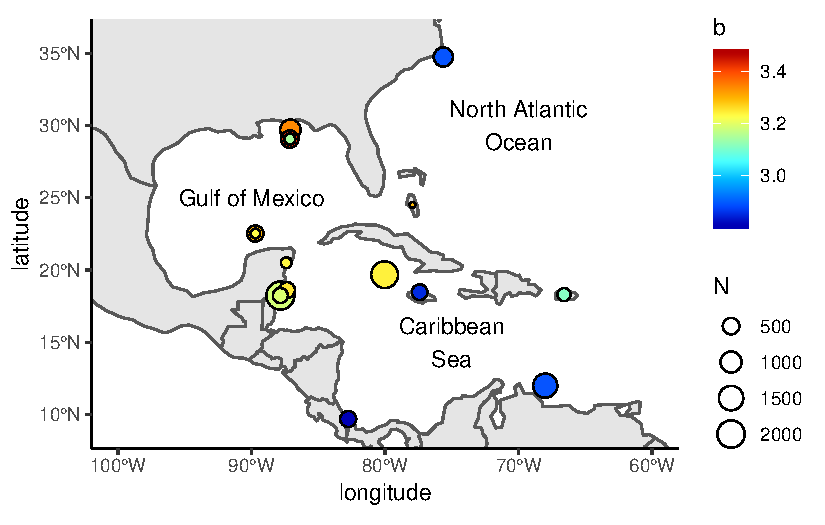
\includegraphics{Manuscript_files/figure-latex/unnamed-chunk-2-1.pdf}
\caption{\label{fig:map}Locations where allometric growth parameters of
lionfish (\emph{Pterois spp}) have been reported. Circle sizes indicate
sample size from each study, colors indicate the \(b\) coefficient from
Eq. \ref{eq:allometric}.}
\end{figure}

We also collected data from 10 sampling sites along the central Mexican
Caribbean coast in 2010 (Supplementary Table 1). Sampling locations
included wall and carpet reefs at depths between 5.7 m and 38.1 m. All
observed lionfish (n = 109) were collected using hand nets and numbered
collection bottles. The use of hand nets prevented any weight loss due
to bleeding and allowed better representation of small sizes by
eliminating gear selectivity. Organisms were euthanized via pithing and
Total Length (TL; mm) and Total Weight (TW; g) were recorded.

The weight-at-length relationship for lionfish in the central Mexican
Caribbean was calculated with the allometric growth function:

\begin{equation}
\label{eq:allometric}
TW = aTL^b
\end{equation}

Where \(a\) is the ponderal index and \(b\) is the scaling exponent or
allometric parameter. Transforming this equation via base-10 logarithms
we obtain:

\begin{equation}
\label{eq:log-alo}
log_{10}(TW) = b\times log_{10}(TL) + log_{10}(a)
\end{equation}

This can be simplified and re-written as:

\begin{equation}
\label{eq:log-alo-trans}
Y = bX + c
\end{equation}

Where \(Y = log_{10}(TW)\), \(X = log_{10}(TL)\), and
\(c = log_{10}(a)\). The coefficients (\(c\) and \(b\)) were estimated
with an Ordinary Least Squares Regression and heteroskedastic-robust
standard error correction \citep{zeileis_2004}. When the \(b = 3\), it
is said that the organism exhibits a perfect isometric growth, so the
\(b\) coefficient was tested against the null hypothesis of isometric
growth (\emph{i.e.} \(H_0: b = 3\)). Coefficients were tested with a
two-tailed Student's t, and the significance of the regression was
corroborated with an F-test.

Some of the reviewed studies inconsistently defined \(a\) as either the
ponderal index from Eq. \ref{eq:allometric} or the y-intercept (\(c\))
from Eq. \ref{eq:log-alo-trans}. Other studies incorrectly reported
parameters as mm-to-g conversions when they were in fact cm-to-g
conversions. We standardized each study by converting coefficients and
report all parameters as TL(mm) to TW (gr) conversions. Locations where
allometric studies have been performed are shown in Figure \ref{fig:map}
and summarized in Table \ref{tab:all_params}.

We obtained a total of 18 parameter pairs by combining length-weight
parameters extracted from the literature and the additional pair
calculated here. We used the central Mexican Caribbean as a case study
of how the use of \emph{ex situ} parameters influences the accuracy of
weight estimates for lionfish. We estimated TW from the TL observations
we collected in the central Mexican Caribbean (n = 109) using each of
the 18 parameter pairs and divided predicted weights by known observed
weights to obtain a simple measure of over- or underestimation.
Difference in mean weight ratios across the different parameter pairs
were tested with a one-way analysis of variance (ANOVA) and Tukey's test
was used for \emph{post-hoc} tests. All analyses were performed in R
version 3.5.0 \citep{rcore_2018}. Raw data and code used in this work
are available on github.

\section{Results}\label{results}

The length-weight relationship for organisms from the central Mexican
Caribbean resulted in the coefficient values
\(a = 3.2056297\times 10^{-6}\), \(b = 3.2347391\) and
\(c = -5.4940866\) (\(R^2 = 0.977\), F(df = 1; 107) = 6928.67,
\(p < 0.001\)). The allometric factor (\(b\)) was significantly
different from \(b = 3\) (\(t(107) = 6.04; p<0.001\)) indicating that
lionfish present allometric growth. The length-weight coefficients
estimated in this study were within the range identified by studies in
other regions (Table \ref{tab:all_params}). Figure \ref{fig:l-w-carib}
shows the relationship between TL and TW for this region, and model fit
statistics are presented in Table \ref{tab:reg_table}.

\begin{figure}
\centering
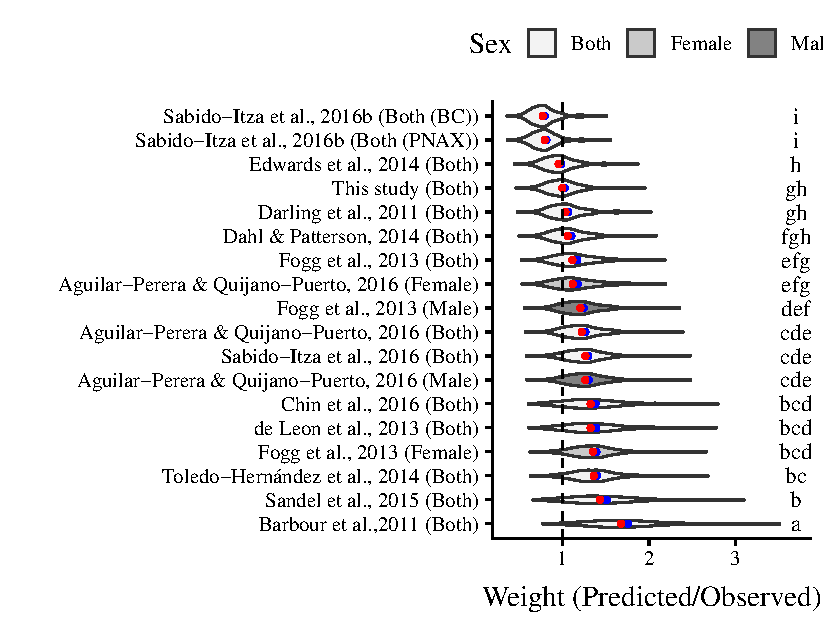
\includegraphics{Manuscript_files/figure-latex/unnamed-chunk-7-1.pdf}
\caption{\label{fig:l-w-carib}Length-weight relationship for 109
lionfish sampled in the central Mexican Caribbean. Points indicate
samples, dashed black line indicates curve of best fit, marginal plots
represent the density distribution of each variable.}
\end{figure}

\begin{table}[!htbp] \centering 
  \caption{\label{tab:reg_table}Coefficients of the linear model fit to Eq \ref{eq:log-alo-trans}. Numbers in parenthesees represent heteroskedastic-robust standard errors.} 
  \label{} 
\begin{tabular}{@{\extracolsep{5pt}}lc} 
\\[-1.8ex]\hline 
\hline \\[-1.8ex] 
 & \multicolumn{1}{c}{$log_{10}(TW)$} \\ 
\cline{2-2} 
\hline \\[-1.8ex] 
 c & $-$5.494 (0.083)$^{***}$ \\ 
  b & 3.235 (0.039)$^{***}$ \\ 
 \hline \\[-1.8ex] 
F Statistic & 6928.67*** (df = 1; 107) \\ 
Observations & 109 \\ 
Adjusted R$^{2}$ & 0.976 \\ 
Residual Std. Error & 0.096 (df = 107) \\ 
\hline 
\hline \\[-1.8ex] 
\textit{Note:}  & \multicolumn{1}{r}{$^{*}$p$<$0.1; $^{**}$p$<$0.05; $^{***}$p$<$0.01} \\ 
\end{tabular} 
\end{table}

There were significant differences in our predicted weights for the
central Mexican Caribbean when using the different pairs of parameters
(\(F(df = 17; 1944) = 61.55; p < 0.001\)). The lowest weight estimates
resulted from using the allometric parameters from Banco Chinchorro in
the Caribbean, with mean \(\pm\) SD of 40.37 \(\pm\) 58.74 gr
\citep{sabidoitz_2016}, and the highest weight estimates came from the
Northern Atlantic with 73.76 \(\pm\) 96.11 gr \citep{barbour_2011}. To
put this in context, true observed weights were 52.56 \(\pm\) 76.58 gr.
These correspond to predicted-to-observed weights ratios of 0.80 \(\pm\)
0.19 and 1.76 \(\pm\) 0.50 (mean \(\pm\) SD), respectively.

The calculated ratio of predicted-to-observed weight ranged from 0.36 to
3.51, indicating that \emph{ex situ} parameters can result in major
under- and overestimations. Tukey's \emph{post-hoc} test suggests that
weight ratios for the central Mexican Caribbean were not different from
those obtained with parameters from Little Cayman, the Bahamas, and some
sites in the Gulf of Mexico (Tukeys HSD \(p > 0.05\)). Weight estimates
using parameters from the Gulf of Mexico and North-Western Atlantic were
higher on average than those from the Caribbean (Fig
\ref{fig:all_allo}). The average (\(\pm\) SD) predicted-to-observed
weight ratios from these three regions were 1.24 \(\pm\) 0.309, 1.76
\(\pm\) 0.496, and 1.17 \(\pm\) 0.398, respectively.
Predicted-to-observed weight ratios are presented in Figure
\ref{fig:bio_ratio}. Spineless weight parameters from \citet{fogg_2013}
still produced predicted-to-observed weight ratios \textgreater{} 1.

\begin{table}

\caption{\label{tab:unnamed-chunk-9}\label{tab:all_params}Summary of 18 allometric growth parameters available for lionfish in the invaded range from peer-reviewed literature and this study. All parameters have been adjusted to convert from millimeters to grams. n = Sample size, Sex specifies whether data was presented for Females (F), Males (M), or both genders combined (B), a = scaling parameter for Eq. 1 (presented in $\times 10^{-5}$), c = y-intercept for Eq. 3, b = exponent or slope for Eq. 1 or Eq. 3, respectively. The Fit column contains the reported $R^2$ of the model fit.}
\centering
\begin{tabular}[t]{l|l|l|l|r|r|l|l}
\hline
Region & Sex & n & a & b & c & Fit & Reference\\
\hline
Caribbean & B & 458 & 3.6 & 2.81 & -4.44 & - & Sandel et al., 2015\\
\hline
Caribbean & B & 419 & 2.8 & 2.85 & -4.56 & 0.8715 & Chin et al., 2016\\
\hline
Caribbean & B & 1450 & 2.3 & 2.89 & -4.64 & 0.96 & de Leon et al., 2013\\
\hline
Caribbean & B & 1887 & 0.3 & 3.24 & -5.52 & 0.97 & Edwards et al., 2014\\
\hline
Caribbean & B & - & 0.25 & 3.29 & -5.60 & - & Darling et al., 2011\\
\hline
Caribbean & B & 2143 & 0.52 & 3.18 & -5.28 & 0.9907 & Sabido-Itza et al., 2016\\
\hline
Caribbean & B & 227 & 0.8 & 3.11 & -5.10 & 0.958 & Toledo-Hernández et al., 2014\\
\hline
Caribbean & B & 449 & 0.23 & 3.25 & -5.64 & 0.97 & Sabido-Itza et al., 2016b\\
\hline
Caribbean & B & 368 & 0.32 & 3.19 & -5.50 & 0.98 & Sabido-Itza et al., 2016b\\
\hline
Caribbean & B & 109 & 0.32 & 3.23 & -5.49 & 0.9766 & This study\\
\hline
GoM & B & 934 & 0.21 & 3.34 & -5.68 & 0.98 & Dahl \& Patterson, 2014\\
\hline
GoM & B & 472 & 0.29 & 3.30 & -5.54 & 0.95 & Aguilar-Perera \& Quijano-Puerto, 2016\\
\hline
GoM & F & 67 & 0.12 & 3.47 & -5.93 & 0.95 & Aguilar-Perera \& Quijano-Puerto, 2016\\
\hline
GoM & M & 59 & 0.42 & 3.23 & -5.38 & 0.95 & Aguilar-Perera \& Quijano-Puerto, 2016\\
\hline
GoM & B & 582 & 0.14 & 3.43 & -5.86 & 0.99 & Fogg et al., 2013\\
\hline
GoM & M & 119 & 0.27 & 3.31 & -5.57 & 0.97 & Fogg et al., 2013\\
\hline
GoM & F & 115 & 0.68 & 3.14 & -5.17 & 0.94 & Fogg et al., 2013\\
\hline
North Atlantic & B & 774 & 2.9 & 2.89 & -4.54 & - & Barbour et al., 2011\\
\hline
\end{tabular}
\end{table}

\begin{figure}
\centering
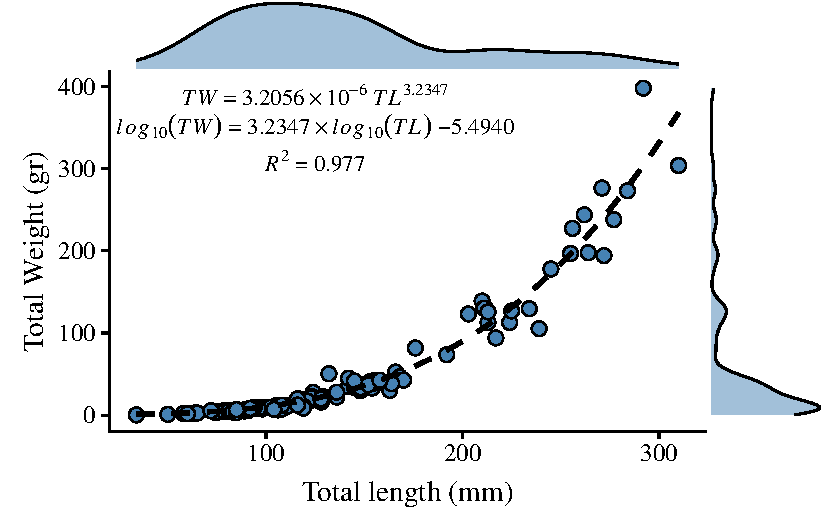
\includegraphics{Manuscript_files/figure-latex/unnamed-chunk-11-1.pdf}
\caption{\label{fig:all_allo}Length-weight relationships (n = 18) for 12
studies and this study. Colors indicate studies from which the
parameters were extracted. Dotted, dashed and solid lines show models
for males, females, and combined sexes, respectively. The dashed black
line represents the relationship estimated in this study.}
\end{figure}

\begin{figure}
\centering
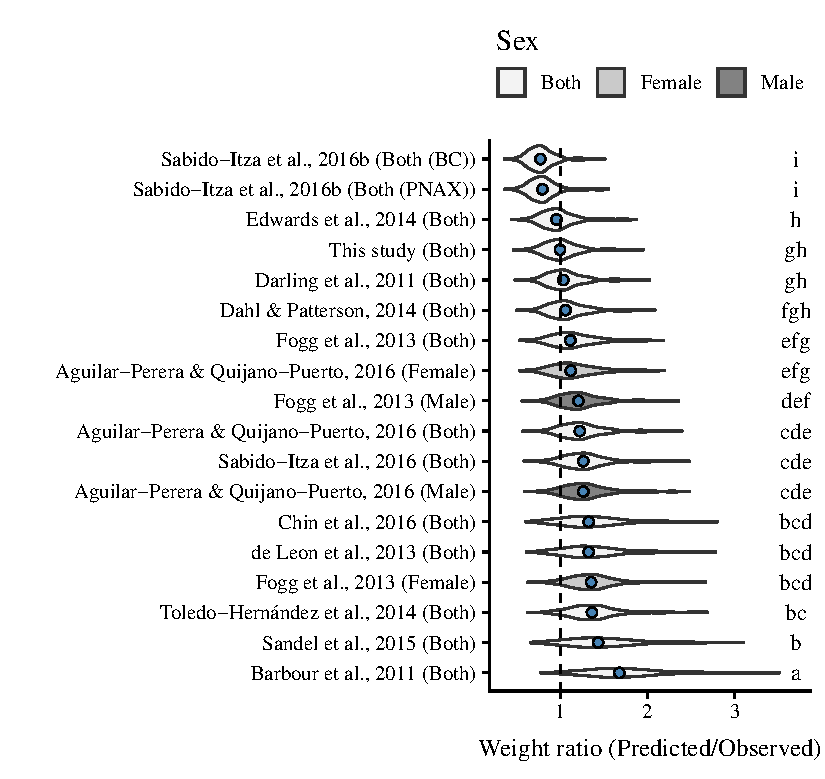
\includegraphics{Manuscript_files/figure-latex/unnamed-chunk-13-1.pdf}
\caption{\label{fig:bio_ratio}Violin plot of predicted-to-observed
weight ratios for 18 pairs of allometric parameters. Blue circles
indicate median values and Like letters indicate values that do not
differ significantly.}
\end{figure}

\clearpage

\section{Discussion}\label{discussion}

We detected substantial differences in weight-at-length between
organisms from the Caribbean, Gulf of Mexico, and North-Western
Atlantic. Groupings of predicted-to-observed weight ratios aligned with
the spatial distribution of the examined studies, suggesting that these
differences are mediated by space. These regional allometric differences
mirror similar patterns in age-at-length of lionfish across both their
invaded and native regions \citep{pusack_2016}. Variation may be driven
by genetics or by organisms' exposure to distinct environmental
conditions. For example, \citet{betancurr_2011} used mitochondrial DNA
to demonstrate the existence of two distinct population groups,
identified as the ``Caribbean group'' and ``Northern Group'', and
\citet{fogg_2015} alternatively suggested that age-at-length differences
may be climate-driven. Differences in weight-at-length could also
reflect differential energy input or usage, or a combination of both.
Future research is needed to determine which processes are at work here.

Differences in length-weight relationships have traditionally been
highlighted as potential pitfalls to fishery management. For example,
\citet{wilson_2012} show that small-scale variations in length-at-age
and fishing mortality in other Scorpaeniformes translate to differential
landings, effort, and catch per unit effort in the live fish fishery of
California, and that these differences must be taken into account in
management plans. The lionfish case poses the opposite scenario, where
the manager desires to eradicate species. To accurately gauge both the
effectiveness of lionfish removal efforts and the resources needed to
successfully manage an invasion, we must acknowledge and understand
regional biological differences in important variables such as
allometric growth parameters.

The results presented here have major implications for management. For
example, \citet{edwards_2014} simulated a lionfish culling program under
two scenarios, one using length-at-age and length-to-weight parameters
from North Carolina and one using parameters from Little Cayman. Their
results show that using different parameters caused up to a four-year
difference in the time required for the simulated lionfish population to
recover to 90\% of its initial biomass after removals ceased. Here, we
show that using one set of length-weight parameters versus another for a
given length can result in more than a threefold under- or
overestimation of total weight. These spatially-driven differences
become especially important when allocating resources for lionfish
removal programs, incentivizing lionfish fisheries as a source of
alternative livelihoods, or estimating ecosystem impacts. Research
efforts focused on invasive lionfish populations need to use parameters
calculated for their region to the extent possible, or at least use
reasonable sets of different parameters that provide upper and lower
bounds in their results.

\section{Acknowledgements}\label{acknowledgements}

The authors would like to thank thank Nils Van Der Haar and Michael
Doodey from Dive Aventuras as well as Guillermo Lotz-Cador who provided
help to collect samples.

Conflict of Interest: The authors declare that they have no conflict of
interest.

\bibliographystyle{spbasic}
\bibliography{references.bib}

\end{document}
